\documentclass[conference]{IEEEtran}
\IEEEoverridecommandlockouts

% Packages
\usepackage{amsmath}
\usepackage{graphicx}
\usepackage{float}
\usepackage{listings}
\usepackage[utf8]{inputenc}
\usepackage{cite}   % Para las citas [1], [2]
\usepackage[T1]{fontenc}
\usepackage{hyperref}
\usepackage{amssymb}
\usepackage{booktabs}
\usepackage{array}    % For \newcolumntype
\newcolumntype{L}{>{$}l<{$}} % Define a left-align math-mode column
% ...existing code...
% added: TikZ for diagrams
\usepackage{tikz}
\usetikzlibrary{arrows.meta, positioning, shapes, calc, backgrounds, automata}
\usepackage{pgfplots}
\pgfplotsset{compat=1.18}
\usepackage{enumitem}
\usepackage{caption}
\usepackage{subcaption}
% ...existing code...

\begin{document}

\title{Robotics 2025}

\author{%
\IEEEauthorblockN{Ismael González Loro, Samuel Corrionero Fernández, José Pulido Delgado}
\IEEEauthorblockA{\textit{Ingeniería Informática en Ingeniería de Computadores} \\
	extit{Universidad de Extremadura}\\
Cáceres, Spain \\
Email: \{igonzaleoa, scorrion, jopulidod\}@alumnos.unex.es}\\
\url{https://github.com/CoferSamuel/ODFE_robotica}
}

\maketitle
\sloppy

\begin{abstract}
This paper is a summary of the Robotics 2025 subject. It presents theory lessons given in class and the development and implementation of a reactive control system for the OmniRobot platform. The system was implemented using a Component-Based Software Engineering (CBSE) paradigm, leveraging the open-source RoboComp framework. The architecture, written in C++, includes a Qt-based graphical user interface for high-level control and monitoring. The system's effectiveness was validated through a series of tasks, e.g., "Sweeping a room" and "Coordinate system based on global coordinates". The results demonstrate that the CBSE approach significantly simplified development and debugging, leading to a robust and maintainable robotic system. This paper provides a practical validation of the RoboComp framework for building complex, reactive applications.
\end{abstract}

\begin{IEEEkeywords}
Mobile robotics, Component-Based Software Engineering, RoboComp, Webots, C++, Simulation, Reactive systems
\end{IEEEkeywords}

\section{Introduction}
The field of mobile robotics studies machines capable of autonomous motion through dynamic environments. According to Corke \cite{corke2011robotics}, mobile robots range from simple reactive platforms such as Elsie the tortoise to complex deliberative systems like Shakey, the first robot capable of reasoning about its environment. These contrasting paradigms—reactive and deliberative—have shaped modern robot control architectures \cite{brooks1986robust, thrun2005probabilistic}. Murphy \cite{murphy2000introduction} highlights this dichotomy as one of the defining distinctions between artificial intelligence (AI) and engineering approaches to robotics: the former focuses on adaptability and autonomy, while the latter emphasizes precision and repeatability.

Historically, robotics evolved along two separate trajectories: industrial manipulators and AI-driven autonomous systems. Industrial robots prioritized accuracy and control theory for repetitive tasks in structured environments, while AI robotics pursued intelligent perception and decision-making for unstructured contexts such as space exploration \cite{murphy2000introduction}. The convergence of these paths—industrial precision with AI adaptability—has become the foundation of modern mobile robotic design.

In recent years, the convergence of Component-Based Software Engineering (CBSE) and robotic simulation has transformed how robotic systems are developed and tested. Frameworks like RoboComp \cite{rodriguez2011robocomp} allow developers to design modular components that encapsulate specific functionalities such as perception, actuation, or control. This modularity accelerates development, enhances code reuse, and facilitates integration between heterogeneous systems. As Murphy \cite{murphy2000introduction} observes, this modular approach echoes the AI field’s long-standing goal of creating autonomous agents composed of interacting intelligent subsystems (e.g., perception, planning, reasoning, and learning).

The project described in this paper was carried out within an academic environment aimed at providing students with practical experience in mobile robot software engineering. Using the RoboComp framework, a reactive control system was implemented for the OmniRobot platform, a simulated differential-drive robot in Webots. The robot is equipped with sensors (e.g., LiDAR) and actuators managed through interconnected software components. This aligns with Murphy’s concept of \textit{teleoperation transitioning to autonomy}, where systems evolve from human-supervised control toward self-governing behavior through improved perception and decision mechanisms.

Following the principles discussed by Corke \cite{corke2011robotics} and Murphy \cite{murphy2000introduction}, this project adopts a reactive navigation approach, where the robot continuously perceives and responds to its surroundings. The main objective is to demonstrate the effectiveness of CBSE methodologies in building modular, maintainable, and extensible robotic systems. The rest of this paper describes the technical setup, tools, and methodologies used to achieve these goals.

% --- Subsección de tipos de robots ---
\subsection{Types of Robots}
\label{sec:robot_types}

Robots can be broadly categorized based on their intended environment and method of locomotion. While hybrid designs exist, this subsection outlines four primary types that form the basis for most robotic systems.

\subsubsection{Mobile Robots (Wheeled)}
These robots navigate the ground using wheels, as seen in Fig.~\ref{fig:mobile_robot}. They are the most common type in industrial and domestic settings due to their high energy efficiency, stability, and mechanical simplicity. They are foundational to logistics and manufacturing, excelling on flat or semi-structured surfaces for tasks like material transport. Their primary limitation is a reliance on prepared environments, as they struggle to traverse unstructured terrain, stairs, or significant obstacles.

\begin{itemize}
    \item \textbf{Representative Example:} Warehouse Robot (e.g., Amazon Kiva \cite{amazon_robotics}).
\end{itemize}

\begin{figure}[H]
    \centering
    \includegraphics[width=0.9\columnwidth]{multimedia/introduction/robots/mobile_robot.png}
    \caption{A typical wheeled mobile robot \cite{amazon_robotics}.}
    \label{fig:mobile_robot}
\end{figure}

\subsubsection{Aerial Robots (Drones)}
Commonly known as drones, these robots operate in the air, typically using a multi-rotor configuration (like the quadcopter in Fig.~\ref{fig:aerial_robot}) for high maneuverability and vertical takeoff. Their key advantage is the ability to access a three-dimensional workspace, providing an aerial perspective for tasks like infrastructure inspection, precision agriculture, search and rescue, and cinematography. Key engineering challenges for this class include limited flight time due to battery constraints, payload capacity, and navigating complex, often regulated, airspace.

\begin{itemize}
    \item \textbf{Representative Example:} Quadcopter (e.g., DJI Phantom \cite{dji_phantom}).
\end{itemize}

\begin{figure}[H]
    \centering
    \includegraphics[width=0.9\columnwidth]{multimedia/introduction/robots/aerial_robot.png}
    \caption{A quadcopter, a common type of aerial robot \cite{dji_phantom}.}
    \label{fig:aerial_robot}
\end{figure}

\subsubsection{Legged Robots}
These robots use articulated limbs (legs) for movement, mimicking biological locomotion. This design, seen in quadrupeds (Fig.~\ref{fig:legged_robot}) or bipeds, allows them to traverse complex, unstructured, and human-centric environments (like stairs) that are inaccessible to wheels. They offer high mobility and adaptability by stepping over obstacles and adjusting their gait. Primary applications include remote inspection in hazardous areas, disaster response, and research. However, they face significant challenges in dynamic stability, control complexity, and lower energy efficiency compared to wheeled systems.

\begin{itemize}
    \item \textbf{Representative Example:} Boston Dynamics' Spot \cite{boston_spot}.
\end{itemize}

\begin{figure}[H]
    \centering
    \includegraphics[width=0.9\columnwidth]{multimedia/introduction/robots/legged_robot.png}
    \caption{The 'Spot' quadruped legged robot \cite{boston_spot}.}
    \label{fig:legged_robot}
\end{figure} 

\subsubsection{Aquatic Robots}
These robots are designed for operation in or on water (Fig.~\ref{fig:aquatic_robot}). They are broadly classified into Autonomous Underwater Vehicles (AUVs), which are untethered and perform pre-programmed missions, and Remotely Operated Vehicles (ROVs), which are tethered to a human operator for real-time control. Applications include oceanographic research, seafloor mapping, offshore infrastructure maintenance, and underwater archaeology. Key challenges involve waterproofing, resistance to high pressure, and the need for alternative navigation and communication systems (e.g., acoustic modems), as GPS and radio waves are ineffective underwater.

\begin{itemize}
    \item \textbf{Representative Example:} Underwater ROV \cite{videoray_rov}.
\end{itemize}

\begin{figure}[H]
    \centering
    \includegraphics[width=0.9\columnwidth]{multimedia/introduction/robots/aquatic_robot.png}
    \caption{An aquatic robot (ROV) for underwater tasks \cite{videoray_rov}.}
    \label{fig:aquatic_robot}
\end{figure}

\section{Materials and Methods}

\subsection{Component-Based Software Engineering (CBSE)}
Component-Based Software Engineering (CBSE) is a paradigm that promotes the development of software systems through the integration of reusable, self-contained components. Each component exposes defined interfaces and encapsulates its internal functionality \cite{szyperski2002component}. In robotics, CBSE has become essential due to the inherent complexity and multidisciplinary nature of robotic systems \cite{brugali2015software}.

RoboComp is an open-source framework designed to support CBSE in robotics. It provides communication middleware based on Ice (Internet Communications Engine), enabling distributed components to interact seamlessly \cite{rodriguez2011robocomp}. This architecture promotes scalability, allowing different robotic subsystems (e.g., navigation, perception, planning) to run independently while sharing data through well-defined interfaces. Such modularity reduces integration costs and facilitates code reuse across different robotic projects.

The CBSE paradigm also aligns with Model-Driven Engineering (MDE) practices, emphasizing the use of high-level abstractions for system design and implementation. In educational contexts, CBSE provides a valuable learning platform, enabling students to experiment with distributed architectures and system integration within a controlled simulation environment.

\subsection{Development Environment and Technical Resources}
The development process was carried out in a simulated environment using Webots \cite{michel2004cyberbotics}, a professional mobile robot simulator that allows realistic testing of control algorithms before deployment. The programming languages used were C++ \cite{stroustrup2013cpp}, with build automation handled by CMake \cite{hoffman2003cmake}. Source code management was performed using GitHub, fostering collaborative development and version control \cite{bird2011github}.

The use of simulation and modular software engineering reflects the pedagogical goals discussed by Murphy \cite{murphy2000introduction}, who emphasized the importance of bridging teleoperation principles with autonomy in educational robotics. Students are encouraged to iterate between manual control and autonomous modes, observing how layered control architectures respond to dynamic environments—paralleling the historical evolution from telemanipulators to intelligent mobile robots.


\begin{itemize}
    \item \textbf{Operating system:} The project was developed on Linux, specifically Ubuntu-based distributions, due to their strong support for open-source robotics software. Linux provides native compatibility with essential libraries such as ROS, RoboComp, and CMake. Its terminal-based workflow facilitates dependency management and compilation processes. Furthermore, Linux’s permission and process control systems enhance robustness and security in real-time applications \cite{quigley2009ros}.
    
    \item \textbf{Class PC (Sala Beta):} Intel(R) Core(TM) i9-9900K CPU @ 3.60GHz; Kingston 16GB \(x2\) (lab machine used for in-class development and tests).

    \item \textbf{Programming language:} C++23. C++ is a general-purpose language designed by Bjarne Stroustrup as an enhancement of the C language. It supports multiple paradigms (procedural, object-oriented, and generic programming), offering both high-level abstraction and low-level hardware control \cite{stroustrup2013cpp}. Over time, C++ has evolved through international standardization, maintaining backward compatibility while introducing features that enhance expressiveness and safety. Its large community ensures extensive documentation and continuous innovation. In robotics, C++ is preferred due to its efficiency, strong typing, and deterministic performance in real-time systems.

    \item \textbf{Framework:} Qt6 was used to develop graphical user interfaces (GUIs) and handle event-driven programming. Qt6 offers cross-platform support, an extensive widget library, and native integration with CMake, facilitating visualization and control panels for robotics. In this project, Qt6 supported the interface components of RoboComp and simplified interaction with robot control modules.

    \item \textbf{Version control platform:} GitHub was used for distributed version control and team collaboration. Through branching and merging mechanisms, it allowed contributors to develop features concurrently while maintaining synchronization. Continuous Integration (CI) workflows were configured to automate compilation and testing. GitHub also supports code reviews and issue tracking, facilitating agile and traceable development practices \cite{bird2011github}.
    
    \item \textbf{Build automation system:} CMake was used as the build automation and configuration tool. CMake simplifies the process of building multi-platform projects by generating native build systems such as Makefiles. It also allows dependency management through configuration files (\texttt{CMakeLists.txt}). In robotics, CMake’s modularity aligns with CBSE principles, enabling separate component compilation and linking \cite{hoffman2003cmake}.
    
    \item \textbf{Integrated development environment:} Visual Studio Code (VSCode) and CLion were used. VSCode is a lightweight, cross-platform IDE developed by Microsoft, offering extensions for C++, Git integration, and debugging tools. Its open-source nature and extensibility make it ideal for collaborative robotics development. CLion, developed by JetBrains, provides intelligent code analysis, CMake integration, and refactoring tools. It enables in-depth static code analysis and real-time syntax inspection, which reduce debugging time and improve code quality. The IDEs enhanced productivity by providing syntax highlighting, linting, and build management integrated with RoboComp’s component structure.
    
    \item \textbf{Simulation software:} Webots is a professional-grade robot simulator that allows the modeling and control of robots in a 3D virtual environment \cite{michel2004cyberbotics}. It supports sensors, actuators, and physics simulation, enabling rapid prototyping without the need for physical robots. Webots provides interfaces for C++, Python, and ROS, making it suitable for educational and research applications. In this project, Webots was used to simulate the OmniRobot platform and its environment, providing realistic testing conditions for perception and control algorithms.
    
    \item \textbf{Robotic components utilized:}
    
    \textbf{- OmniRobot}: The sweeping robot, named OmniRobot, is modeled as a circular platform equipped with distributed sensors. It features a minimalist white design and a tall structure supported by four small omnidirectional wheels capable of linear and rotational motion. At the top of the robot, there is a tray to transport objects. It was provided by the professor and developed by the RoboComp team. \\
    \textbf{- Lidar3D}: This component simulates a LiDAR sensor capable of measuring both the distance and angular position of nearby obstacles. It provides 360° environmental awareness, essential for obstacle avoidance and mapping. It was provided by the professor and developed by the RoboComp team. \\
    \textbf{- Chocachoca}: Software responsible for controlling OmniRobot’s motion behavior, acting as the robot’s decision-making brain. It defines navigation and collision-avoidance behaviors based on sensor inputs. This is the only component created by the authors, following the professor’s guidelines. \\
    \textbf{- Webots-bridge}: Serves as the intermediary communication layer between OmniRobot, Lidar3D, and Chocachoca, allowing seamless data exchange within the simulation environment. \\
    \textbf{- JoystickPublish}: Connects a real joystick to OmniRobot, enabling manual control during testing phases. It was provided by the professor and developed by the RoboComp team. \\
    \textbf{- Aspirator}: A program with a GUI that evaluates the efficiency of the robot in terms of surface coverage and time employed.

    \textbf{- rcnode}: This tool provides a publish-subscribe messaging infrastructure for RoboComp components to communicate asynchronously. Components can publish messages to topics and subscribe to topics of interest, enabling decoupled, event-driven communication in robotic systems.  

        % Removed duplicate static component_diagram image; replaced later with inline TikZ

% ...existing code...
        \begin{figure}[H]
            \centering
%            \includegraphics[width=0.4\textwidth]{multimedia/others/component_diagram.png}
%            \caption{Component diagram}
%            \label{fig:comp_dia}
%
% replaced above static image with inline TikZ diagram:
            \resizebox{\columnwidth}{!}{%
            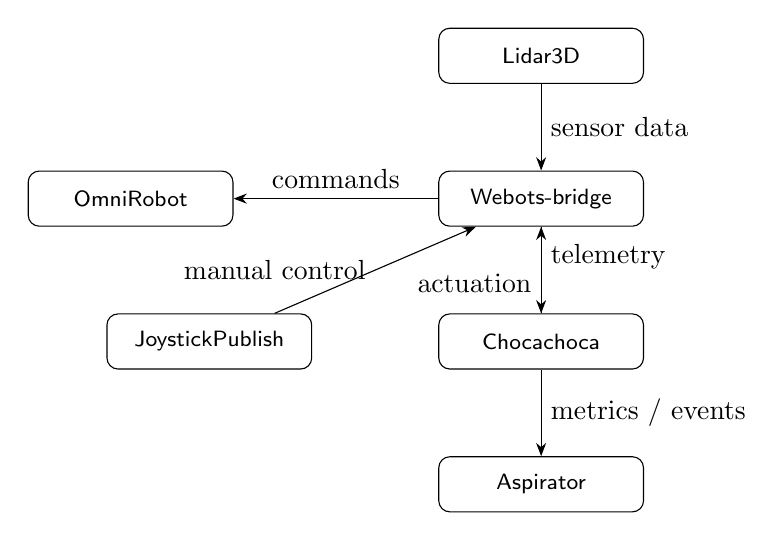
\begin{tikzpicture}[
                % reduced spacing and sizes for a smaller diagram
                node distance=11mm and 16mm,
                comp/.style={draw, rectangle, rounded corners, minimum width=26mm, minimum height=7mm, align=center, font=\sffamily\footnotesize},
                >=Stealth
            ]
                % Nodes
                \node[comp] (omni) {OmniRobot};
                \node[comp,right=of omni, xshift=10mm] (web) {Webots-bridge};
                \node[comp, above=of web] (lidar) {Lidar3D};
                \node[comp, below=of web] (choca) {Chocachoca};
                \node[comp, left=of choca] (joy) {JoystickPublish};
                \node[comp, below=of choca] (asp) {Aspirator};

                % Connections
                \draw[->] (lidar) -- (web) node[midway, right] {sensor data};
                \draw[->] (web) -- (omni) node[midway, above] {commands};
                \draw[->] (web) -- (choca) node[pos=0.35, right] {telemetry};
                \draw[->] (choca) -- (web) node[pos=0.35, left] {actuation};
                \draw[->] (joy) -- (web) node[pos=0.5, left] {manual control};
                \draw[->] (choca) -- (asp) node[midway, right] {metrics / events};

            \end{tikzpicture}%
            }
            \caption{Component diagram}
            \label{fig:comp_dia}
        \end{figure}

    \item \textbf{Documentation tool:} Overleaf was used for collaborative documentation and paper writing. Overleaf is a cloud-based LaTeX editor that simplifies academic and technical writing through real-time synchronization, version history, and multi-user editing. Its compatibility with IEEE templates facilitates the production of professional papers and ensures reproducible document formatting.
\end{itemize}

\section{Activity 1: Sweeping Robot}

\subsection{Objective}
The main objective of this activity is to design and implement a program (Chocachoca) that guides an autonomous robot capable of covering the largest possible area within a confined space in the shortest time. The system relies on sensor feedback (Lidar3D) to detect obstacles and dynamically adjust its trajectory to achieve efficient coverage while avoiding collisions. Performance is evaluated in a test lasting up to 3 minutes using the previously described Aspirator component.

\subsection{Graphical User Interface (GUI)}
The GUI provides real-time visualization of the robot's perception and localization state, enabling monitoring and debugging of the control system during operation.

\begin{figure}[H]
    \centering
    \fbox{\includegraphics[width=0.82\columnwidth]{multimedia/task1/GUI.png}}
    \caption{Real-time GUI showing LiDAR point cloud visualization and robot localization.}
    \label{fig:gui_chocachoca}
\end{figure}

The interface displays two key components:

\begin{itemize}
    \item \textbf{LiDAR Point Cloud Visualization:} The pink/red dotted outline represents the filtered LiDAR 3D point cloud, which shows the detected obstacles and environment geometry in real-time. The raw sensor data undergoes two filtering stages to reduce noise and improve computational efficiency: (1) angle-based grouping reduces the point cloud by selecting, for each azimuth direction, only the closest detected point; and (2) isolation filtering removes sparse, noise-prone points that lack neighboring detections within a 200 mm radius. This two-stage filtering preserves the geometric structure of the environment while eliminating spurious measurements. The maximum sensing range is limited to 12 meters to balance perception coverage with real-time processing requirements.

    \item \textbf{Robot Representation:} The blue square in the center of the visualization represents the robot's current position and orientation within the environment. Its location is updated continuously from the robot's odometry system, which tracks the robot's x and z Cartesian coordinates (in millimeters) and heading angle alpha (in radians). This visualization provides immediate feedback on the robot's self-reported localization state, enabling real-time monitoring of whether the robot is executing the intended trajectory and responding correctly to obstacle avoidance commands.
\end{itemize}

\subsection{Operational Algorithms and Behavioral States}
As previously explained, the robot’s navigation behavior is defined by a finite set of operational states that govern its decision-making process and movement patterns, as shown in Figure \ref{fig:stateMachine}.

\begin{figure}[H]
    \centering
    \includegraphics[width=0.9\columnwidth]{multimedia/task1/stateMachine/stateMachine.png}
    \caption{State machine for the Chocachoca controller.}
    \label{fig:stateMachine}
\end{figure}

        

The initial state is \textit{SPIRAL}, in which the robot performs a spiral movement until it approaches an obstacle. It then transitions to \textit{TURN} to avoid the obstacle. After turning, the robot randomly switches to either \textit{FORWARD} or \textit{FOLLOW\_WALL}.

If it switches to \textit{FORWARD}, it will continue moving straight until it encounters another obstacle, at which point it transitions back to \textit{TURN}. Otherwise, it changes to \mbox{\textit{FOLLOW\_WALL}}, where the robot moves parallel to the wall.

All states are detailed below:


% (Previously defined in preamble)
\begin{table}[H] % [H] requires the 'float' package
\centering
\caption{Variable and Constant Legend}
\label{tab:var_legend}
\begin{tabular}{L l}
\toprule
\textbf{Variable} & \textbf{Description} \\
\midrule
D_T & Min. distance to obstacle to trigger \textit{TURN}. \\
v_s & Robot's forward speed during \textit{SPIRAL}. \\
\omega_s & Robot's rotational speed during \textit{SPIRAL}. \\
V_{s,max} & Max. allowed forward speed in \textit{SPIRAL}. \\
\omega_{min} & Min. allowed rotational speed (0 rad/s). \\
V_{max} & Max. general forward speed (\textit{FORWARD}/\textit{TURN}). \\
c & Counter for "stuck" iterations in \textit{TURN}. \\
d_{min} & Data point for the closest detected obstacle. \\
D_S & Distance threshold to switch to \textit{SPIRAL}. \\
v & Calculated forward speed in \textit{FORWARD}. \\
d & Specific distance value of the closest obstacle. \\
T_{min} & Min. safety threshold for speed calculations. \\
v_b & Calculated braking speed. \\
B_{max} & Max. allowed braking value. \\
\omega & Calculated rotational speed (\textit{TURN}/\textit{FORWARD}). \\
\bottomrule
\end{tabular}
\end{table}

\subsubsection{SPIRAL} Executes an Archimedean spiral trajectory to maximize surface coverage, gradually increasing the radius of rotation while avoiding overlaps in path. The transition between spiral and turn states is determined by the following conditions:
\begin{itemize}
    \item 1.1. Check for nearby obstacles: if any obstacle is within $D_T$, abort spiral and change to \textit{TURN}.
    \begin{align}
        D_T &= 600.0 \ \text{mm} \label{eq:m_d_t}
    \end{align}
    \item 1.2. If no obstacles, slowly increase advance speed ($v_s$) and reduce rotation ($\omega_s$) to expand the spiral.
    \begin{align}
        v_s &= 500.0 \ \text{mm/s} \\
        \omega_s &= 3.0 \ \text{rad/s}
    \end{align}
    These values change as follows:
    \begin{align}
        v_s &\mathrel{+}= 2.5 \ \text{mm/s} \\
        \omega_s &\mathrel{-}= 0.01 \ \text{rad/s}
    \end{align}
    Respecting the thresholds:
    \begin{align}
        V_{s,max} &= 1000.0 \ \text{mm/s} \\
        \omega_{min} &= 0.0 \ \text{rad}
    \end{align} 
\end{itemize}

\subsubsection{TURN} Rotate the robot in place to avoid obstacles that are blocking its path. The robot keeps turning until the frontal area is clear, then decides whether to go forward or follow a wall.

\begin{itemize}
    \item 1. Filter frontal points
        \begin{itemize}
            \item Select only points in $\pm 45^\circ$ frontal cone
            \item Determines if path ahead is clear
        \end{itemize}
    \item 2. Find nearest frontal obstacle
        \begin{itemize}
            \item Find the closest point in front of the robot
        \end{itemize}
    \item 3. Decision tree: Clear path vs Still blocked
        \begin{itemize}
            \item Path A: Obstacle cleared
                \begin{itemize}
                    \item Check if nearest obstacle $> 700$ mm
                    \item Randomly set rotation speed:
                    
                    - 0.6 rad/s with a 70\%
                    
                    - 3.0 rad/s with a 30\%
                    
                    \item Randomly choose next state: \textit{FOLLOW\_WALL} or \textit{FORWARD} with $V_{max}$ speed.
                    \begin{align}
                        V_{max} &= 800 \text{ mm/s} \label{eq:max_adv}
                    \end{align}
                    \item Randomness avoids deterministic loops
                \end{itemize}
            \item Path B: Still blocked
                \begin{itemize}
                    \item Increment $c$. This variable measure the amount of times that the robot executes \textit{TURN} in the Path B.
                    \item If $c \ge 100$, force positive rotation (escape hatch)
                    \item Otherwise, choose rotation direction based on obstacle side.
                    \item This path is usually seen in the corners and this approach achieves to escape from them when stuck.
                \end{itemize}
        \end{itemize}
\end{itemize}

\subsubsection{FORWARD} Commands linear motion until an obstacle is detected by the front sensors.
\begin{itemize}
    \item 1. Collect frontal points: keep points with $\phi$ between $-45$\textdegree{} and $+45$\textdegree{}.
    \item 2. Find the closest frontal point.
    \item 3.1. If $d_{min} > D_S$ (very far):
    \begin{align}
        D_S &= 2000 \ \text{mm}
    \end{align} 
    \begin{itemize}
        \item Switch to \textit{SPIRAL} state.
    \end{itemize}
    \item 3.2. Else: $d_{min}$ is closer
    \begin{itemize}
        \item 3.2.1. If the distance to $d_{min}$ from the robot is greater than $D_T$ \eqref{eq:m_d_t}, keep \textit{FORWARD} with a new value of $v$ and zero rotation.

        $v$ will increase until the distance to the point is equal or smaller than $D_T$ \eqref{eq:m_d_t}. It has to increase gradually, because the virtual robot is simulating a real robot with real physics.
        
    \begin{align}
        v = (d_{min} - T_{min}) \cdot \frac{V_{max}}{D_T - T_{min}}
    \end{align}
    
        % This formula can be illustrated using the following graphic (Fig. \ref{fig:adv_speed}):

        % \begin{figure}[H]
        %     \centering
        %     \includegraphics[width=0.4\textwidth]{multimedia/task1/formulas/fw_speedup.png}
        %     \caption{adv\_speed}
        %     \label{fig:adv_speed}
        %  \end{figure}
        
        
        \item 3.2.2. Else, transition to \textit{TURN} with linear $0$ and a new value of rotation $\omega$.
        Compute brake term $v_b$ proportional to how much closer than $D_T$ \eqref{eq:m_d_t} we are:
        
            \begin{align}
                v_b &= (D_T - d_{min}) \cdot \frac{B_{max}}{D_T - T_{min}} \label{eq:brake_orig}\\
                	\text{Let } x &:= D_T - d_{min},\qquad y := v_b \nonumber\\
                y &= \frac{B_{max}}{D_T - T_{min}}\,x \;=\; m\,x + n \label{eq:brake_linear}
            \end{align}

            \noindent Where:
            \begin{itemize}
                \item $m = \dfrac{B_{max}}{D_T - T_{min}}$ (slope / proportional gain),
                \item $n = 0$ (no intercept when using $x=D_T-d_{min}$).
            \end{itemize}

            \noindent The first line (Eq.~\ref{eq:brake_orig}) shows the original brake expression. Using $x=D_T-d_{min}$ yields the linear form (Eq.~\ref{eq:brake_linear}). Here $x$ is the distance-to-threshold scalar and $y$ is the brake term $v_b$ (both in consistent units). These are control variables, not spatial robot coordinates.

            \begin{figure}[H]
                \centering
                \includegraphics[width=0.65\columnwidth]{multimedia/task1/formulas/brake_law.png}
                \caption{Brake law: linear relation $y=mx+n$ where $x = D_T - d_{min}$, $y = v_b$, $m = B_{max}/(D_T - T_{min})$, and $n = 0$. Thresholds at $x=0$ (obstacle trigger $d_{min}=D_T=600$ mm) and $x=D_T-T_{min}$ (safety threshold) are shown as dashed gray lines.}
                \label{fig:brake_plot}
            \end{figure}

            %  This can be represented graphically by the next graphic (Fig. \ref{fig:brake_speed}):

            % \begin{figure}[H]
            % \centering
            % \includegraphics[width=0.4\textwidth]{multimedia/task1/formulas/fw_braking.png}
            % \caption{brake\_speed}
            %  \label{fig:brake_speed}
            %  \end{figure}
            
            Finally, assign the angular speed:
            \begin{align}
                \omega = v_b / 2 
            \end{align}
            The /2 is just a tuning factor to make the rotation speed reasonable. Without it, the robot might spin too fast.
    \end{itemize}
\end{itemize}

\subsubsection{FOLLOW\_WALL} Implements wall-following using proportional control to maintain a constant distance from the wall.

\begin{itemize}
    \item 1. Compute the absolute closest point among all points (not only frontal).
    \begin{itemize}
        \item $d_{min} = \text{min\_element(points, by p.r)}$; this is interpreted as the wall (closest obstacle).
    \end{itemize}
    \item 2. Handle cases depending on the distance to the closest point: $d_{min}$:
    \begin{itemize}
        \item If $D_T \leq r < D_T + 150$:
        \begin{itemize}
            \item Continue in \texttt{FOLLOW\_WALL} with \texttt{adv = 150.0f} and \texttt{rot = 0.0f} (move forward slowly).
            \item This is the “ideal following band”.
        \end{itemize}

        \item If $r > D_T + 150$ (too far from the wall):
        \begin{itemize}
            \item If the angle to $d_{min}$ $\phi < 0$ (wall to the left): continue in \texttt{FOLLOW\_WALL} with speed of \texttt{150 mm/s} and angular speed of \texttt{-0.2 rad/s} (small rotation toward the wall; negative rotation means one direction).
            \item Else (wall to the right): continue in \mbox{\textit{FOLLOW\_WALL}} with speed of \texttt{150 mm/s} and angular speed of \texttt{+0.2 rad/s} (small rotation to the other side).
        \end{itemize}

        \item If $D_T - 100 < r < D_T + 10$ (too close to the wall):
        \begin{itemize}
            \item If $\phi < 0$ (wall is left and near): continue in \texttt{FOLLOW\_WALL} with speed of \texttt{150 mm/s} and angular speed of \texttt{+0.2 rad/s} (steer away).
            \item Else steer away the other side, with same linear speed and the same value of angular speed but with negative rotation.
        \end{itemize}
        \item Else (no special condition matched):
        \begin{itemize}
            \item Fall back to \textit{FORWARD} with linear speed of 600.0 mm/s (fast forward).
        \end{itemize}
    \end{itemize}
    \item 3. The function attempts to maintain the robot in a narrow corridor around $D_T$~\eqref{eq:m_d_t}.
\end{itemize}


These are all the detailed explanations of the states. State transitions are triggered based on sensor input and internal logic thresholds, ensuring adaptive behavior in dynamic environments. The modular implementation enables easy adjustment of thresholds and parameters for different testing scenarios.


\subsection{Experimental Results}
The robot was evaluated in multiple simulated environments in Webots. These environments were provided by Robocomp and are used to test the robot in different contexts. The performance metrics focused on surface coverage efficiency.

\begin{itemize}
    \item \textbf{Test 1}

        This is a simple map with no obstacles, just 4 walls composing a rectangle room (Figure \ref{fig:sw_map}). After several attempts, the best result achieved was 70 \% of the room covered.
        \begin{figure}[H]
            \centering
            \includegraphics[width=0.4\textwidth]{multimedia/task1/results/sw.png}\\[0pt]
            \includegraphics[width=0.4\textwidth]{multimedia/task1/results/sw_test.png}
            \caption{SimpleWorld map and results}
            \label{fig:sw_map}
        \end{figure}

    \item \textbf{Test 2}

        This map is more complex than the previous one. A box is added, increasing the difficulty for the robot to cover the entire floor (Figure \ref{fig:sw1}). The best result accomplished was the 67 \% of the floor covered, worse than the previous one (Figure \ref{fig:sw1}).
        \begin{figure}[H]
            \centering
            \includegraphics[width=0.4\textwidth]{multimedia/task1/results/1box_world.jpeg}
            \includegraphics[width=0.4\textwidth]{multimedia/task1/results/1box_test.jpeg}
            \caption{SimpleWorld map with one box and results}
            \label{fig:sw1}
        \end{figure}

    \item \textbf{Test 3}

    The increasing difficulty continues and now the room has two boxes (Figure \ref{fig:sw2}). In this occassion, the best percentage achieved was 59 \% (Figure \ref{fig:sw2}). As can be observed, the robot performs a bit worse.
        \begin{figure}[H]
            \centering
            \includegraphics[width=0.4\textwidth]{multimedia/task1/results/2box_world.jpeg}
            \includegraphics[width=0.4\textwidth]{multimedia/task1/results/2box_test.jpeg}
            \caption{SimpleWorld map with two boxes and results}
            \label{fig:sw2}
        \end{figure}
\end{itemize}
\subsection{Conclusions}

As shown in the tests, the robot was unable to achieve complete floor coverage in any trial. The best result was obtained in Test 1, where there were no obstacles, while the worst performance occurred in Test 3, which has more obstacles.

The conclusions drawn from this activity are that the robot, with the Chocachoca software, struggles to cover complex rooms with obstacles, and performs better in simpler environments with unobstructed layouts.

% Activity 2: Robot Self-Localization in the Room (revised)
\section{Activity 2: Robot Self-Localization in the Room}

\subsection{Objective}
The primary objective of Activity 2 is to design and implement a geometry-based Localiser for the OmniRobot. This component enables the robot to estimate and incrementally correct its pose within a known rectangular room, effectively compensating for odometry drift.

The system operates by detecting salient corners from 2D LiDAR scans and associating them with the room’s nominal corners using the Hungarian assignment algorithm. Based on these correspondences, it computes small incremental translation and rotation corrections by solving a linearized least-squares system.

Integrated into the RoboComp architecture, the Localiser operates in two distinct modes:
\begin{itemize}
    \item \textbf{Estimation-only:} The system runs with actuators disabled to evaluate localization accuracy in isolation.
    \item \textbf{Closed-loop:} The system provides corrected pose estimates to the reactive controller developed in Activity 1, enabling more accurate navigation.
\end{itemize}

Quantitative evaluation is conducted in the Webots simulation environment through multiple randomized trials. To assess system performance, we measure the accuracy of the estimated pose (deviation of positional and angular errors), the speed of correction  and the robustness of the algorithm.


Figure \ref{fig:problem_viz} visualizes the localization problem. The lines represent where the robot expects the walls to be, while the dots show where the LiDAR sensor actually detects them. The misalignment between the two indicates that the robot's estimated position is incorrect due to accumulated movement errors. The Localiser works to align these two views, correcting the robot's position.

\begin{figure}[H]
    \centering
    \includegraphics[width=0.4\textwidth]{multimedia/task2/Captura desde 2025-11-11 12-55-57.png}
    \caption{Visualization of the localization problem.}
    \label{fig:problem_viz}
\end{figure}

\subsection{Proposed Solution and Methodology}



\subsubsection{Proposed Solution}
The Localiser is a modular system that corrects the robot's position using 2D LiDAR data. In every control cycle, it calculates how much the robot has drifted from its expected position in the room and applies a correction.

The process follows these steps:
\begin{enumerate}
  \item \textbf{Preprocess scans:} We filter the LiDAR data to keep only the closest points and remove noise. This ensures we work with clean data.
  
  \item \textbf{Extract lines (RANSAC):} We use the RANSAC algorithm to find straight lines in the point cloud. These lines correspond to the walls of the room.

    \begin{figure}[H]
        \centering
        \includegraphics[width=0.4\textwidth]{multimedia/task2/1761190966479.jpg}
        \caption{RANSAC Line Extraction}
        \label{fig:ransac_viz}
    \end{figure}
  
  \item \textbf{Find corners:} We look for intersections between perpendicular lines to find the corners of the room. We verify these corners and remove duplicates.


  \item \textbf{Transform model corners:} We need to compare the known map of the room with what the robot is currently seeing. Since the map is fixed and the robot is moving, we mathematically transform the map's corners to the robot's point of view.
  
  If the robot is at position $T$ and rotated by $\theta$, we calculate the local position of a map corner $C_{map}$ as:
  \[ C_{local} = R(\theta)^T (C_{map} - T) \]
  This formula subtracts the robot's position and rotates the point, allowing us to directly match the map against the LiDAR data.

  \item \textbf{Match corners (Hungarian):} We use the Hungarian algorithm to match the detected corners with the known map corners based on distance. This tells us which detected corner corresponds to which map corner.

    \begin{figure}[H]
        \centering
        \includegraphics[width=0.2\textwidth]{multimedia/task2/5.png}
        \caption{Hungarian Matching}
        \label{fig:hungarian_viz}
    \end{figure}

  \item \textbf{Optional consensus filter:} To avoid errors, we can use a secondary check to remove matches that don't fit well with the others.

  \item \textbf{Compute and apply pose update:} Using the matched corners, we calculate the exact error in the robot's position (x, y, and angle) and apply a correction to fix it.
\end{enumerate}

\subsubsection{Measurement Protocol and Metrics}
\textbf{Experimental Setup:}
\begin{itemize}
  \item \textbf{Environments:} We use the same Webots simulation environments as in Activity 1.
  \item \textbf{Trials:} We run at least 10 randomized trials for each scenario. In each trial, the robot starts at a random position.
  \item \textbf{Modes:} We test the system in two modes:
    \begin{itemize}
        \item \textit{Estimation-only:} The robot does not move, to test localization accuracy.
        \item \textit{Closed-loop:} The robot moves using the corrected position, to test navigation performance.
    \end{itemize}
\end{itemize}

\textbf{Data Logging:}
We record key data at every step to analyze performance, including the true position, estimated position, number of detected corners, and calculation time.

\textbf{Primary Metrics:}
\begin{itemize}
  \item \textbf{Positional Error:} The distance between the estimated position and the true position.
  \item \textbf{Angular Error:} The difference between the estimated angle and the true angle.
  \item \textbf{Convergence Time:} How long it takes for the robot to find its correct position (error < 0.5 m).
  \item \textbf{Valid-solve Rate:} How often the system successfully calculates a position correction.
  \item \textbf{Solver Latency:} The time it takes to compute the solution.
\end{itemize}



\subsection{Mathematical Techniques}

\subsubsection{Rigid Transforms in SE(2)}
To compare the map with the sensor data, we need to express them in the same coordinate system. A point $C$ in the world frame can be transformed to the robot's frame using the robot's position $T$ and rotation matrix $R(\theta)$:
\[
\tilde C \;=\; R(\theta)^\top (C - T)
\]
This equation essentially "moves" the map points so they are relative to the robot.

\subsubsection{Small-Angle Linearization}
The relationship between the robot's position and the sensor measurements is non-linear (due to sine and cosine functions), which makes it hard to solve directly. However, since we correct the position frequently, the errors are small. This allows us to use a mathematical trick called linearization ($\cos\Delta\theta\approx 1, \sin\Delta\theta\approx \Delta\theta$) to turn the problem into a system of linear equations:
\[
\begin{aligned}
\tilde C_x &\approx T_x + m_x - \Delta\theta\,m_y \\
\tilde C_y &\approx T_y + m_y + \Delta\theta\,m_x
\end{aligned}
\]
Now we can solve for the corrections using standard linear algebra.

\subsubsection{Solving the Linear System}
We stack the equations from all matched corners into a large system $W r = b$. To find the best correction $r$ (change in x, y, and angle), we use the Singular Value Decomposition (SVD) method. SVD is robust and helps us find the optimal solution that minimizes the overall error between the expected and actual corner positions.

\subsubsection{Robust Line Extraction (RANSAC)}
RANSAC is an algorithm used to find lines in noisy data. It works by:
\begin{enumerate}
  \item Randomly picking two points to define a line.
  \item Counting how many other points fit this line (inliers).
  \item Repeating this many times and keeping the line with the most inliers.
\end{enumerate}
This ensures we find the actual walls and ignore scattered noise points.

\subsubsection{Corner Detection}
Corners are found by intersecting the lines detected by RANSAC. An intersection is considered a valid corner if:
\begin{itemize}
  \item The lines are perpendicular (forming a 90-degree angle).
  \item The intersection point actually lies within the wall segments.
\end{itemize}
We also filter out duplicate corners to ensure a clean set of features.
\subsubsection{Data Association (Hungarian Algorithm)}
Once we have the corners from the map and the corners from the LiDAR, we need to match them. We use the Hungarian algorithm, which finds the optimal pairing that minimizes the total distance between matched corners. This ensures we are comparing the right corner in the map to the right corner in the sensor data.

\subsubsection{Outlier Rejection}
Even with good matching, mistakes can happen. We use a consensus filter (similar to RANSAC) to double-check the matches. It looks for a group of matches that all agree on the same robot position and discards any "outliers" that don't fit this consensus. This prevents a single bad match from ruining the position correction.


\subsubsection{Outlier Rejection}
Even with good matching, mistakes can happen. We use a consensus filter (similar to RANSAC) to double-check the matches. It looks for a group of matches that all agree on the same robot position and discards any "outliers" that don't fit this consensus. This prevents a single bad match from ruining the position correction.

\subsection{Experimental Results}
The robot was evaluated in multiple simulated environments in Webots provided by RoboComp.

\textbf{Test Case 1: SimpleWorld}
The first test environment (Figure \ref{fig:sw_map_res}) consists of a simple rectangular room with no obstacles.

Figure \ref{fig:sw_test_res} presents the results of the localization process. The image shows two perspectives:
\begin{itemize}
    \item On the left, the \textbf{robot's internal view}, where the detected corners (from LiDAR) are successfully matched with the map corners. The visual alignment confirms that the algorithm has correctly estimated the robot's pose.
    \item On the right, the \textbf{external simulation view}, showing the actual position of the robot in the room.
\end{itemize}
The successful matching of corners in the internal view corresponds to the accurate positioning seen in the external view, validating the system's performance.

\begin{figure}[H]
    \centering
    \includegraphics[width=0.45\textwidth]{multimedia/task2/Imagen pegada.png}
    \caption{SimpleWorld Map}
    \label{fig:sw_map_res}
\end{figure}

\begin{figure}[H]
    \centering
    \includegraphics[width=0.45\textwidth]{multimedia/task2/Imagen pegada (2).png}
    \caption{SimpleWorld Test Results}
    \label{fig:sw_test_res}
\end{figure}

A video demonstration of the localiser in action can be viewed at:
\begin{center}
\url{https://drive.google.com/file/d/1f_QV6La_op_kgW51XC4HKma_aQV0oxyi/view?usp=sharing}
\end{center}

\subsection{Conclusions}
This activity successfully integrates a geometry-based Localiser into the RoboComp architecture. The developed pipeline (using RANSAC, Hungarian algorithm, and SVD) effectively corrects the robot's position in rectangular environments.

While the system performs well in simple scenarios, it requires robust filtering to handle complex environments with obstacles. Future improvements could include more advanced optimization techniques or combining data from multiple sensors to further increase reliability.



% Activity 3: Visually-guided navigation (II). Finding doors
\section{Activity 3: Visually-guided navigation (II). Finding doors}

\subsection{Objective}
The primary objective of this task is to extend the robot's navigation capabilities to include autonomous door detection and traversal, enabling transition between distinct rooms. The system must implement a robust feature extraction algorithm based on 2D LiDAR range-bearing vectors to identify closed doors within the environment. A Finite State Machine (FSM) will orchestrate the navigation tasks. The sequence commences at an assumed target in the room's geometric center, where the Localiser developed in Activity 2 is deployed to refine the robot's pose. Subsequently, the control logic involves: detecting the door's patch, navigating to a 1-meter standoff position, aligning the robot's heading with the opening, and cross at the other room.

\subsection{Behavioral States}
As explained previously, robot navigation behavior is defined by a finite set of operational states that govern its decision-making process and movement patterns, as shown in Figure \ref{fig:door_fsm_tikz}.
    \begin{figure}[H]
        \centering
        % Mantengo la escala y el tamaño de letra, solo cambio distancias
        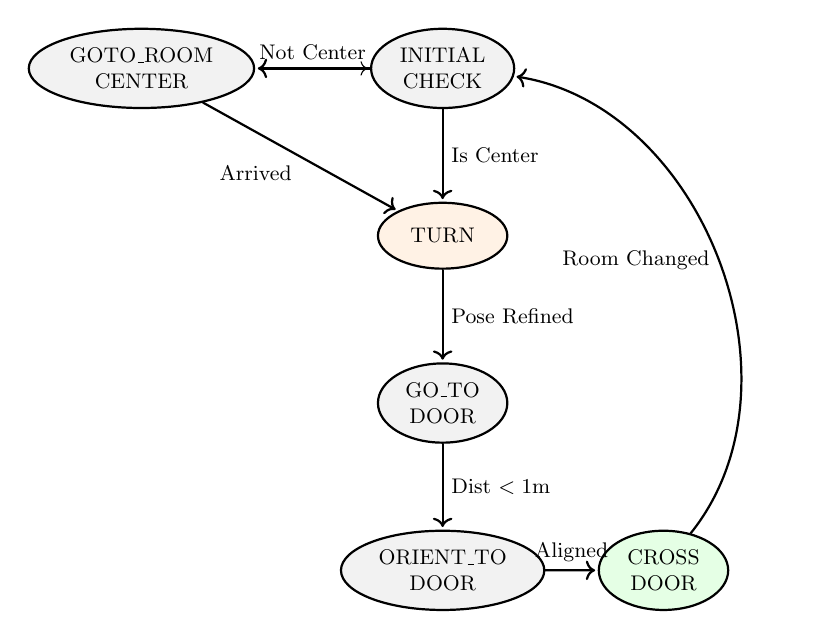
\begin{tikzpicture}[scale=0.85, transform shape, shorten >=1pt, node distance=2.5cm, on grid, auto]
            
            \tikzset{
                customState/.style={draw, ellipse, thick, minimum height=2.8em, minimum width=5.5em, align=center, fill=gray!10, font=\small},
                acceptState/.style={draw, ellipse, thick, minimum height=2.8em, minimum width=5.5em, align=center, fill=green!10, font=\small},
                initialState/.style={draw, ellipse, thick, minimum height=2.8em, minimum width=5.5em, align=center, fill=white, font=\small}
            }
            
            % Nodos (Estados)
            \node[customState, initial, initial text=] (s0) {INITIAL\\CHECK};
            
            % --- CAMBIO AQUÍ: Aumentado a 5cm para dejar espacio a "Not Center" ---
            \node[customState] (s1) [left=4.5cm of s0] {GOTO\_ROOM\\CENTER};
            
            \node[customState, fill=orange!10] (s2) [below=2.5cm of s0] {TURN};
            
            \node[customState] (s3) [below=2.5cm of s2] {GO\_TO\\DOOR};
            
            \node[customState] (s4) [below=2.5cm of s3] {ORIENT\_TO\\DOOR};
            
            % Ajustado también abajo a 5cm para mantener la simetría
            \node[acceptState] (s5) [right=3.3cm of s4] {CROSS\\DOOR};
    
            % Transiciones
            \path[->, thick, font=\small]
            % Ahora hay espacio de sobra para esta etiqueta:
            (s0) edge node [above] {Not Center} (s1) 
            (s0) edge node [right] {Is Center} (s2)
            (s1) edge node [below left] {Arrived} (s2)
            (s2) edge node [right] {Pose Refined} (s3)
            (s3) edge node [right] {Dist $< 1$m} (s4)
            (s4) edge node [above] {Aligned} (s5)
            (s5) edge [bend right=60] node [left] {Room Changed} (s0);
            
        \end{tikzpicture}
        \caption{Finite State Machine (FSM) logic for the door crossing task.}
        \label{fig:door_fsm_tikz}
    \end{figure}

    The process initiates in the \textit{INITIAL\_CHECK} state, where the system verifies if the robot is positioned at the room's geometric center. If the robot is not centered, it transitions to \textit{GOTO\_ROOM\_CENTER} to navigate to the optimal starting position. Once the center is reached—or if the robot was already positioned there—the system changes to \textit{TURN}.
    
    In this state, the robot performs an in-place rotation until the LiDAR detects the target patch. Upon successful detection, it transitions to \textit{GOTO\_DOOR}, navigating towards the door located behind the identified patch. When the robot approaches within a 1-meter threshold of the entrance, it switches to \textit{ORIENT\_TO\_DOOR} to align its heading with the door frame. Finally, once alignment is confirmed, the state changes to \textit{CROSS\_DOOR} to traverse the opening, after which the cycle restarts for the new room.
    \vspace{0.5cm} All states are detailed below:


    \subsubsection{GO\_TO\_ROOM\_CENTER} Navigation behavior is encapsulated in the \texttt{goto\_room\_center} method, which operates as a closed-loop controller. The routine requires a valid target coordinate, representing the room's geometric center relative to the robot's current frame.
    
    The control logic proceeds as follows:
    \begin{enumerate}
        \item \textbf{Distance Computation:} At each time step, the Euclidean distance $d$ to the target is computed as the norm of the relative position vector $\mathbf{p}_{target}$:
        \begin{equation}
            d = \|\mathbf{p}_{target}\|
        \end{equation}
        \item \textbf{Termination Condition:} A proximity threshold $\delta$ is defined at $100$ mm. If the distance to the target falls below this threshold ($d < \delta$), the maneuver is considered complete. The robot sets its velocities to zero, resets the target variable, and triggers a state transition to \texttt{TURN}.
        
        \item \textbf{Velocity Command:} If the threshold is not met, the target vector is passed to the \texttt{robot\_controller} \cite{siegwart2011intro}, which calculates the required linear ($v$) and angular ($\omega$) velocities. These commands are then sent to the omnidirectional base platform to drive the robot towards the centroid.
    \end{enumerate}

    \subsubsection{TURN}
    The \texttt{turn} state implements an active perception strategy designed to locate specific visual landmarks (colored panels) within the environment. This method executes a scanning maneuver in which the robot performs a constant-velocity rotation at the place ($\omega = 0.2$ rad/s) while simultaneously processing visual data from the RGB camera.
    
    The logic operates as follows:
    \begin{enumerate}
        \item \textbf{Target Selection:} The routine checks the Boolean flag \texttt{search\_green} to determine the target hue (Green or Red). This allows the same state logic to be reused for different stages of the mission.
        \item \textbf{Image Processing:} At each iteration, the system queries the \texttt{ImageProcessor::check\_color\_patch\_in\_image} static method. This function performs color segmentation and blob detection on the camera stream, returning a Boolean status indicating if the target patch is centered within the field of view.
        \item \textbf{Termination Condition:} If the target is detected (`detected == true`), the robot immediately arrests its motion by setting all velocity components to zero. The internal flag \texttt{badge\_found} is asserted, and the FSM transitions to the \texttt{GOTO\_DOOR} state, signaling that the orientation phase is complete.
        \item \textbf{Continuous Rotation:} As long as the target remains undetected, the method maintains the rotational velocity command. The kinematic control law governing this state is defined as:
        \begin{equation}
            S_{next} = 
            \begin{cases} 
                \texttt{GOTO\_DOOR} & \text{if } \text{detected} = \text{true} \\
                \texttt{TURN} & \text{otherwise}
            \end{cases}
            \label{eq:turn_logic}
        \end{equation}

    \noindent where $S_{next}$ represents the state at the next instant in time.        
    \end{enumerate}
    
    \subsubsection{GO\_TO\_DOOR}
    The \texttt{Go\_To\_Door} state orchestrates the approach maneuver towards the detected exit while simultaneously computing the precise orientation required for the subsequent alignment phase.
    
    The control logic is divided into two operational stages:
    \begin{enumerate}
    \item \textbf{Target Acquisition and Approach}
    The system continuously queries the \texttt{door\_detector} module. If no valid door candidates are identified within the LiDAR scan, the robot executes a recovery behavior by rotating at a fixed angular velocity ($0.2$ rad/s) to sweep the environment.
    Upon detection, a navigation target $\mathbf{p}_{target}$ is generated at a defined standoff distance ($\delta = 1000$ mm) perpendicular to the door's centroid. This ensures the robot stops with sufficient clearance to perform the final alignment maneuver.
    
    \item \textbf{Alignment Vector Computation \cite{sanderson2016dot}}
    When the robot stops in front of the door ($v \approx 0$), it calculates the correct angle to face the opening. Since a door is detected simply as a line segment, there is a risk that the robot might calculate the angle backwards (facing the room instead of the exit). To fix this $180^\circ$ ambiguity, the system uses the known center of the room as a reference. It calculates a vector pointing away from the room's center to ensure the robot faces the correct direction before trying to cross.

    To resolve this, the system uses the room's geometric center ($\mathbf{c}_{room}$) as a reference anchor. It compares the door's normal vector $\mathbf{n}$ with the vector pointing towards the room center ($\mathbf{v}_{inward}$) using the dot product. If the calculation indicates that the vector points into the room ($\mathbf{n} \cdot \mathbf{v}_{inward} > 0$), the target orientation is flipped to ensure the robot faces the exit:
    
    \begin{equation}
        \mathbf{v}_{target} = 
        \begin{cases} 
        -\mathbf{v}_{door} & \text{if } \mathbf{n} \cdot \mathbf{v}_{inward} > 0 \\
        \mathbf{v}_{door} & \text{otherwise}
        \end{cases}
    \end{equation}
    \noindent where:
    \begin{description}[labelsep=0.4cm] 
        \item[$\mathbf{v}_{target}$] represents the final corrected heading.
        \item[$\mathbf{v}_{door}$] is the initial vector aligned with the door frame.
        \item[$\mathbf{n}$] denotes the door's normal vector.
        \item[$\mathbf{v}_{inward}$] is the reference vector pointing from the robot's position to the room's geometric center.
    \end{description}
    \end{enumerate}

    Finally, this local vector is transformed into a global world angle $\theta_{global}$, which is stored as a "sticky" target. This prevents orientation jitter in the subsequent state. The system then transitions to \texttt{ORIENT\_TO\_DOOR}.

    \subsubsection{ORIENT\_TO\_DOOR}
    The \texttt{orient\_to\_door} state executes a precision rotation maneuver to align the robot's heading with the previously computed trajectory vector. This decoupling of target computation (performed in \texttt{GO\_TO\_DOOR}) and execution ensures stability, as the target angle remains fixed ("sticky") regardless of sensor noise during the rotation.
    
    The control loop functions as follows:
    \begin{enumerate}
        \item \textbf{State Validation:} The system first validates the existence of the stored \texttt{orient\_target\_angle}. This acts as a safety interlock; if the target is undefined, the system aborts to an safe state.
        \item \textbf{Angular Error Computation:} The current global heading $\theta_{curr}$ is extracted from the robot's rotation matrix. The error $\theta_{err}$ is computed and, crucially, normalized to the range $(-\pi, \pi]$ to correctly handle the trigonometric discontinuity at $\pm 180^\circ$:
        \begin{equation}
            \theta_{err} = \text{atan2}(\sin(\theta_{target} - \theta_{curr}), \cos(\theta_{target} - \theta_{curr}))
        \end{equation}
        \begin{description}[labelsep=0.4cm] 
            \item[$\theta_{err}$] represents the normalized angular error bounded within $(-\pi, \pi]$
            \item[$\theta_{target}$] is the desired orientation (the "sticky" target) computed in the previous state
            \item[$\theta_{curr}$] denotes the robot's current instantaneous heading in the world frame.
        \end{description}

        \item \textbf{Bang-Bang Control Law \cite{alhumairi2019bang}:} Unlike the approach phase, the alignment uses a constant-velocity controller to ensure consistent turning behavior. The control output $\omega_{z}$ is determined by the sign of the error:
        \begin{equation}
            \omega_{z} = -\text{sgn}(\theta_{err}) \cdot \omega_{fixed}
        \end{equation}
        \begin{description}
            \item[$\omega_{fixed}$]  is set to $0.2$ rad/s.
        \end{description}
        \item \textbf{Convergence:} The maneuver terminates when the absolute heading error falls within a tolerance window $\epsilon = 0.2$ rad ($\approx 11.5^\circ$). Upon convergence, the robot halts ($\omega_{z} = 0$), clears the sticky target, and transitions to the subsequent state (e.g., \texttt{CROSS\_DOOR}).
    \end{enumerate}

    \subsubsection{CROSS\_DOOR}
    The final stage of the sequence, \texttt{Cross\_Door}, executes a ballistic (open-loop) maneuver to traverse the physical threshold of the doorway. Unlike previous states that rely on continuous sensor feedback, this state assumes the heading alignment performed in \texttt{ORIENT\_TO\_DOOR} is sufficiently precise to allow a straight-line traversal. This approach minimizes the risk of oscillatory behavior caused by sensor noise within the narrow door frame.
    \vspace{0.5cm}
    The execution logic is time-based rather than geometric:
    \begin{enumerate}
        \item \textbf{Temporal Initialization:} Upon entering the state, a monotonic clock timestamp $t_{start}$ is captured. This ensures the maneuver has a fixed temporal reference frame.
        \item \textbf{Constant Velocity Command:} The robot applies a constant longitudinal velocity $v_{x}$ while maintaining zero lateral and rotational velocities. This enforces a straight trajectory:
        \begin{equation}
            \mathbf{v}_{lineal} = 400\text{ mm/s}
        \end{equation}
        \item \textbf{Termination and Context Switch:} The system calculates the elapsed time $\Delta t = t_{now} - t_{start}$ at each control cycle. The maneuver terminates when $\Delta t$ exceeds a pre-defined safety duration ($T_{limit} = 5.0$ s).
        \item \textbf{Room Transition:} Upon timeout, the robot halts, resets the timer, and executes the \texttt{switch\_room()} routine. This function updates the robot's topological belief (switching the active map or reference frame) before transitioning the FSM to \texttt{GO\_TO\_ROOM\_CENTER} to begin operation in the new environment.
    \end{enumerate}

    \subsubsection{MOTION CONTROLER (Velocity Computation)}
    To guide the robot towards specific spatial targets (e.g., room center or door approach points), a closed-loop kinematic controller was implemented. This module takes the target coordinates $\mathbf{t} = (t_x, t_y)$ expressed in the robot's local reference frame and computes the coupled linear ($v$) and angular ($\omega$) velocities.
    
    \vspace{0.1cm}
    
    The control law prioritizes orientation over translation to ensure smooth natural motion. It uses a Gaussian function to suppress linear velocity when the heading error is large, forcing the robot to turn before accelerating.

    \vspace{0.1cm}
    
    \textbf{1. Angular Control:}
    The angular error $\theta_e$ is computed from the target coordinates. The rotational velocity command is generated using a proportional controller with a high gain ($K_\omega = 0.8$) to ensure fast alignment:
    \begin{equation}
        \omega = K_\omega \cdot \text{atan2}(t_x, t_y)
    \end{equation}
    
    \textbf{2. Linear Control:}
    The linear velocity $v$ is modulated by two distinct factors:
    \begin{itemize}
        \item \textbf{Alignment Factor ($\Omega$)}: A Gaussian function that reduces speed as the alignment error increases. This acts as a "soft" interlock, preventing linear motion during sharp turns.
        \begin{equation}
            \Omega = \exp\left( \frac{-\theta_e^2}{\pi/4} \right)
        \end{equation}
        \item \textbf{Distance Factor ($D$)}: A linear saturation function that creates a smooth deceleration ramp when the robot is within 500 mm of the target, preventing overshoot.
        \begin{equation}
            D = \min\left(1.0, \frac{||\mathbf{t}||}{500}\right)
        \end{equation}
    \end{itemize}
    
    The final linear velocity command is the product of the maximum speed ($V_{max} = 1000$ mm/s) and these modulation factors:
    \begin{equation}
        v = V_{max} \cdot \Omega \cdot D
    \end{equation}    
    \subsection{Experimental Results}
    The proposed navigation system was evaluated within a simulated environment developed in Webots. The testing arena consists of two adjacent rectangular rooms connected by a single, centrally located doorway. Both rooms are devoid of obstacles to isolate the door traversal performance. 
    
    To facilitate the visual recognition task, colored fiducial markers (patches) are aligned with the door frame to guide the robot's approach. The initialization room is characterized by a red marker, while the destination room features a green marker.
    
    Regarding the simulation interface, a real-time Heads-Up Display (HUD) provides critical telemetry data, including the robot's instantaneous linear and angular velocities, as well as the current active state of the Finite State Machine. Additionally, a dynamic plot visualizes the evolution of the minimization error metric throughout the trial.
    
    \vspace{0.1cm}

    % --- PÁGINA 1 ---
    \begin{figure}[H]
        \centering
        \includegraphics[width=1\linewidth]{multimedia/task3/TwoRoomsSimple.png}
        \caption*{ (a) Initial Map Configuration} % Subtítulo manual como tenías
        \caption{Visual comparison of the simulation environment (Part 1).}
        \label{fig:experiment_layout} % Etiqueta de la figura principal
    \end{figure}
    % --- PÁGINA 2 ---
    \begin{figure}[H]
        \ContinuedFloat % Mantiene el número de la figura anterior
        \centering
        \includegraphics[width=1\linewidth]{multimedia/task3/TwoRoomsSimpleResult.png}
        \caption*{ (b) Simulation Result}
        \caption{Simulation result. A full video of the execution is available at: \\ \url{https://drive.google.com/file/d/10n_1iG7BUhLd8JUsoaLkpJoZF9h5ERZR/view?usp=sharing}}
    \end{figure}

  \subsection{Conclusions}
    The proposed system successfully demonstrates the efficacy of a modular Finite State Machine (FSM) for autonomous door traversal. Key contributions include the resolution of the $180^\circ$ directional ambiguity through a geometric dot-product approach referencing the room's centroid, and the implementation of a hybrid control strategy. 
    By decoupling the precise alignment phase (closed-loop) from the traversal phase (open-loop), the system effectively mitigated sensor noise within the narrow doorway. \\
    These results validate the architecture's robustness for reliable topological transitions in multi-room environments.


    % Activity 4: Multi-Room Autonomous Navigation
    \section{Activity 4: Multi-Room Autonomous Navigation}

    \subsection{Objective}
    The primary objective of this task is to extend the robot's navigation capabilities to handle a multi-room environment consisting of two rooms connected by two doors. The system must enable autonomous exploration without requiring a specific starting position, building and maintaining a topological graph map of the environment in real-time.

    \subsection{Ultra-Localiser (Grid Search Bootstrap)}
    A key challenge in multi-room navigation is that the robot may enter a room from any position and orientation. The standard localiser only works when the robot starts at the room center. To solve this, the Ultra-Localiser implements a bootstrap phase using multi-hypothesis grid search.

    \vspace{0.1cm}

    Initial localization facilitates downstream operations. Specifically, approximate positioning is required post-traversal to ascertain which door was crossed and to identify the adjacent rooms linked by that connection.

    \vspace{0.1cm}

    \subsubsection{\textbf{Algorithm Overview}}
    The Ultra-Localiser operates in two phases:
    \begin{enumerate}[label=\alph*)]
        \item \textit{Coarse Localization (Grid Search):} Tests 200 candidate poses across the room:
        \begin{itemize}
            \item $5 \times 5$ spatial grid covering 80\% of the room dimensions
            \item 8 angular orientations (every $45°$)
            \item Total: $25 \times 8 = 200$ hypotheses
        \end{itemize}
        \item \textit{Fine Localization (Incremental SVD):} After bootstrap, the standard pose correction takes over, refining the position each control cycle.
    \end{enumerate}

    \subsubsection{\textbf{Hypothesis Evaluation}}
    For each candidate pose $(x, y, \theta)$, the algorithm:
    \begin{enumerate}[label=\alph*)]
        \item Transforms nominal room corners to the robot frame using the candidate pose:
        \begin{equation}
            \tilde{C} = R(\theta)^\top (C_{world} - T)
        \end{equation}
        where $C_{world}$ is the corner in world coordinates, $T = (x, y)$ is the candidate position, and $R(\theta)$ is the rotation matrix.
        \item Matches detected LiDAR corners against transformed nominal corners using the Hungarian algorithm.
        \item Computes the maximum matching error.
    \end{enumerate}

    The pose with the \textbf{lowest maximum matching error} is selected as the initial robot pose. Localization is considered successful when:
    \begin{itemize}
        \item Match error $< 3500$ mm (configurable threshold)
        \item At least 3 corners are matched
    \end{itemize}

    \begin{figure}[H]
        \centering
        \includegraphics[width=0.9\columnwidth]{multimedia/task4/localised_enteringInRoom1.png}
        \caption{Ultra-Localiser result: Robot successfully localized after entering Room 1 from an arbitrary position.}
        \label{fig:ultra_localiser}
    \end{figure}

    \subsubsection{\textbf{Two-Phase Convergence}}
    The grid search finds the \textit{closest grid point}, not the exact robot position. The incremental solver then refines the pose:

    \begin{table}[H]
    \centering
    \caption{Two-Phase Localization Accuracy}
    \begin{tabular}{lll}
    \toprule
    \textbf{Phase} & \textbf{Function} & \textbf{Accuracy} \\
    \midrule
    Grid Search & Approximate position & Within $\sim$300--500 mm \\
    Incremental SVD & Continuous refinement & Within $\sim$20 mm \\
    \bottomrule
    \end{tabular}
    \end{table}

    \subsubsection{\textbf{Grid Search Mathematics}}
    The search space consists of candidate poses sampled across the room:

    \textbf{Position Grid:}
    \begin{align}
        x_k &\in \{-0.8w, -0.4w, 0, 0.4w, 0.8w\} \\
        y_k &\in \{-0.8l, -0.4l, 0, 0.4l, 0.8l\} \nonumber
    \end{align}

    \textbf{Orientation Set:}
    \begin{equation}
        \theta_k \in \left\{0, \frac{\pi}{4}, \frac{\pi}{2}, \frac{3\pi}{4}, \pi, \frac{5\pi}{4}, \frac{3\pi}{2}, \frac{7\pi}{4}\right\}
    \end{equation}

    For each candidate pose $(x_k, y_k, \theta_k)$, the algorithm computes the maximum matching error:
    \begin{equation}
        E_k = \max_{i \in \text{matches}} \left\| \tilde{C}_i^k - C_i^{detected} \right\|
    \end{equation}

    The optimal initial pose is selected as:
    \begin{align}
        k^* &= \arg\min_k E_k \\
        &\text{subject to: } E_{k^*} < 3500 \text{ mm and } |\text{matches}| \geq 3 \nonumber
    \end{align}

    \subsubsection{\textbf{Incremental Pose Correction}}
    After the grid search bootstrap, the system uses the same SVD-based incremental pose solver described in Activity 2 (Section 2.3). This solver continuously refines the robot's position by solving the linearized least-squares system $Wr = b$ using the pseudoinverse.
    \vspace{0.1cm}
    \subsection{Topological Graph Mapping}
    The robot builds a semantic graph of the environment in real-time, replacing transient decision-making with a persistent memory structure.

    \subsubsection{\textbf{Graph Structure}}
    The graph consists of two types of nodes:
    \begin{itemize}
        \item \textit{ROOM Nodes}: Represent physical rooms (e.g., Room 0, Room 1). Store metadata including dimensions, entry heading, and the ID of the door used to enter.
        \item \textit{DOOR Nodes}: Represent physical connections between rooms. Store geometric endpoints ($p_1$, $p_2$) and their center position.
    \end{itemize}

    \subsubsection{\textbf{Dynamic Construction}}
    \begin{enumerate}
        \item When the robot enters a new room, it calls \texttt{add\_room()}.
        \item Detected doors are added via \texttt{add\_door()} and immediately connected to the current Room node.
    \end{enumerate}

    \subsubsection{\textbf{Topological Linking}}
    The system handles the fact that the same physical door is seen as two different ``Door Nodes'' from different rooms (different coordinates in local frames). When moving from Room A to Room B, the graph \textbf{links} the exit door of Room A to the entry door of Room B:
    \begin{equation*}
        \text{Room\_A} \leftrightarrow \text{Door\_Node\_A} \leftrightarrow \text{Door\_Node\_B} \leftrightarrow \text{Room\_B}
    \end{equation*}

    \subsubsection{\textbf{Exploration State}}
    A door is considered \textbf{Explored} if it has connections to 2 different neighbors (Parent Room + Linked Door). This allows the robot to query unexplored doors and intelligently select new targets, prioritizing unknown areas over backtracking.

    \subsubsection{\textbf{Data Structure}}
    The graph node structure is defined as:
    \begin{lstlisting}[language=C++, basicstyle=\ttfamily\small]
    struct GraphNode {
        int id;
        NodeType type;       // ROOM or DOOR
        Eigen::Vector2f pos; // Center coordinates
        // Room specifics
        int entry_door_id;
        float reference_heading;
        // Door specifics
        Eigen::Vector2f p1, p2;
    };
    \end{lstlisting}

    \begin{figure}[H]
        \centering
        \begin{subfigure}[b]{0.32\columnwidth}
            \includegraphics[width=\textwidth]{multimedia/task4/graph_room0.png}
            \caption{Room 0 recognized}
        \end{subfigure}
        \hfill
        \begin{subfigure}[b]{0.32\columnwidth}
            \includegraphics[width=\textwidth]{multimedia/task4/graph_room1.png}
            \caption{Room 1 recognized}
        \end{subfigure}
        \hfill
        \begin{subfigure}[b]{0.32\columnwidth}
            \includegraphics[width=\textwidth]{multimedia/task4/graph_room0_re-entry.png}
            \caption{Re-entry to Room 0}
        \end{subfigure}
        \caption{Topological graph evolution: (a) Initial state with Room 0 and its 2 doors, (b) After entering Room 1 with door connections established, (c) Re-entry to Room 0 showing complete topology.}
        \label{fig:topo_graph_gui}
    \end{figure}

    \subsection{Door Target Selection Strategy}
    The door selection system uses the topological graph to make intelligent navigation decisions, combining entry identification with a priority-based selection algorithm.

    \subsubsection{\textbf{Entry Door Identification}}
    When the robot enters a room, it must identify which door it came through:
    \begin{itemize}
        \item \textbf{First Visit}: Uses the robot's localized pose to find the closest door (``Proximity'') and registers it as the Entry Door. Crucially, the system \textbf{learns} a bidirectional connection in the Graph between this door and the previous room's exit door.
        \item \textbf{Re-entry}: Uses the \textbf{Learned Connection} from the Graph to identify the entry door instantly. This bypasses proximity checks, making the system immune to localization symmetry errors (e.g., if the robot localizes upside-down due to room symmetry).
    \end{itemize}

    \subsubsection{\textbf{Graph-Based Door Selection (Priority System)}}
    The \texttt{select\_door\_from\_graph()} function implements a priority-based algorithm to choose the next target door:

    \begin{enumerate}
        \item \textit{Priority 1 -- Unexplored, Non-Entry Doors}: The system first searches for doors that are both unexplored (fewer than 2 connections in the graph) AND not the entry door. This prioritizes exploration of new areas while avoiding immediate backtracking.
        
        \item \textit{Priority 2 -- Any Unexplored Door}: If no non-entry unexplored doors exist, the system accepts any unexplored door, even if it is the entry door. This ensures exploration continues.
        
        \item \textit{Priority 3 -- Traversal Logic}: When all doors are explored:
        \begin{itemize}
            \item \textbf{Room 0}: Selects randomly from ALL doors (including the entry door). This prevents deterministic loops and allows the robot to change direction.
            \item \textbf{Room 1+}: Selects only from non-entry doors, ensuring the robot crosses the room rather than immediately returning.
        \end{itemize}
        
        \item \textit{Priority 4 -- Backtrack}: As a last resort (when no other options exist), the robot backtracks through the entry door.
    \end{enumerate}

    \subsubsection{\textbf{Sticky World-Coordinate Tracking}}
    Once a door is selected from the graph, the robot locks onto its world position to prevent target switching during motion:
    \begin{equation}
        P_{world} = R(\theta_{robot}) \cdot P_{local} + T_{robot}
    \end{equation}
    In subsequent control cycles, the system finds the detected door closest to this stored world coordinate, ensuring stable navigation even as the robot moves and the door's apparent position changes in the sensor frame.

    \subsection{Additional Improvements}

    \subsubsection{\textbf{Door Visualization}}
    Detected doors are rendered in the room viewer to provide real-time feedback on the robot's perception:
    \begin{itemize}
        \item \textbf{Cyan lines}: Connect the two endpoints of each detected door, clearly marking the opening.
        \item \textbf{Dark blue circles}: Mark the door endpoints ($p_1$, $p_2$), providing precise visual reference for the door boundaries.
        \item \textbf{Wall projection}: Door endpoints are projected onto the closest wall to ensure consistent geometry and prevent visual artifacts from localization drift.
    \end{itemize}

    The wall projection algorithm works in two steps:
    \begin{enumerate}
        \item \textbf{Find closest wall}: For the door's center point, compute the perpendicular distance to each room wall and select the wall with minimum distance.
        \item \textbf{Project endpoints}: Both door endpoints $p_1$ and $p_2$ are orthogonally projected onto this wall using the formula:
    \end{enumerate}

    Given a wall defined by endpoints $\mathbf{w}_1$ and $\mathbf{w}_2$, the projection of a door endpoint $\mathbf{p}$ onto the wall is:
    \begin{equation}
        \text{proj}(\mathbf{p}) = \mathbf{w}_1 + \frac{(\mathbf{p} - \mathbf{w}_1) \cdot (\mathbf{w}_2 - \mathbf{w}_1)}{||\mathbf{w}_2 - \mathbf{w}_1||^2} (\mathbf{w}_2 - \mathbf{w}_1)
    \end{equation}

    This ensures both door endpoints lie exactly on the wall line, eliminating visual distortions caused by sensor noise or localization inaccuracies.


    \begin{figure}[H]
        \centering
        \includegraphics[width=0.9\columnwidth]{multimedia/task4/doors_drawn.png}
        \caption{Detected doors rendered as cyan lines with dark blue endpoint markers in the room viewer.}
        \label{fig:door_visualization}
    \end{figure}

    \subsubsection{\textbf{GUI Reorganization}}
    The graphical user interface was reorganized to accommodate the new topological graph visualization. The main changes include:
    \begin{itemize}
        \item \textbf{Topological Graph Frame}: New widget added to display Room and Door nodes with their connections in real-time.
        \item \textbf{Camera View Resized}: The panoramic camera view was moved to the bottom-left and reduced in size.
        \item \textbf{Match Error Graph Repositioned}: Moved to share space with the graph frame.
        \item \textbf{Layout Reorganization}: Overall layout adjusted from 4 to 5 main panels.
    \end{itemize}

    \begin{figure}[H]
        \centering
        \includegraphics[width=0.95\columnwidth]{multimedia/task4/fullGUI.png}
        \caption{Updated GUI layout with the new topological graph visualization frame.}
        \label{fig:gui_reorganization}
    \end{figure}

    \subsection{AI Room Number Recognition}
    To enable semantic understanding of the environment, specifically room identification, a deep learning-based perception system was implemented. This system allows the robot to read handwritten digits (0-9) placed on the walls, determining the current room index (e.g., "0" or "1").

    \subsubsection{\textbf{Component Architecture: MNIST Detector}}
    Due to the computational cost of deep neural networks, the recognition logic was decoupled from the main control loop and encapsulated in a dedicated RoboComp component named \texttt{mnist\_detector}. This component, written in Python to leverage the PyTorch ecosystem, communicates with the main C++ controller via the Ice middleware.

    The component exposes a remote interface \texttt{getNumber()}, which returns the verified digit and a confidence score. This asynchronous architecture ensures that the heavy inference tasks do not block the robot's real-time navigation loop. To optimize resources, the component implements a dynamic execution period: it runs at 5 Hz (200 ms) when actively queried by the robot and drops to 0.5 Hz (2000 ms) when idle.

    \subsubsection{\textbf{Neural Network Design and Training}}
    The core of the recognition system is a Convolutional Neural Network (CNN) trained on the MNIST dataset, a standard benchmark consisting of 60,000 training images of handwritten digits.

    The network architecture, implemented using the PyTorch framework, consists of:
    \begin{itemize}
        \item \textbf{Input Layer}: Accepts 28x28 grayscale images.
        \item \textbf{Convolutional Layers}: Two layers (Conv2d) with 32 and 64 filters respectively, using 3x3 kernels and ReLU activation, followed by Max Pooling.
        \item \textbf{Fully Connected Layers}: A dense layer mapping features to 128 neurons, and a final output layer producing probabilities for the 10 digit classes.
    \end{itemize}

    The model was trained offline using the Negative Log Likelihood loss function and the SGD optimizer. The resulting weights were serialized to a \texttt{.pt} file and loaded by the component at runtime.

    \subsubsection{\textbf{Computer Vision Pipeline}}
    Before feeding the image to the neural network, a classic computer vision pipeline is applied to locate and isolate the target numbers within the camera feed:

    \begin{enumerate}
        \item \textbf{ROI Detection}: The system converts the image to HSV color space and applies a red color mask to detect the square badges containing the numbers.
        \item \textbf{Contour Filtering}: Contours are filtered by area and aspect ratio to identify valid candidate frames.
        \item \textbf{Preprocessing}: The region of interest (ROI) is cropped, converted to grayscale, and resized to 28x28 pixels. Crucially, a bitwise inversion is applied to correct the contrast (transforming the white-background real-world image to the black-background format expected by the MNIST-trained model).
        \item \textbf{Inference}: The processed tensor is passed through the CNN, which outputs the most probable digit and its confidence level.
    \end{enumerate}

    This hybrid approach, combining robust color-based segmentation with deep learning classification, provides a reliable mechanism for the robot to semantically ground its location within the topological map.

    \subsection{Experimental Results}
    The multi-room navigation system was evaluated within a simulated environment developed in Webots. The testing arena consists of two adjacent rectangular rooms connected by two distinct doorways, allowing for cyclic navigation patterns. Unlike previous single-door scenarios, this setup tests the robot's ability to handle multiple transition points and re-entry logic.
    
    To facilitate the semantic localization task,  digitsare used as visual markers instead of colored patches. These digits (0-9) are placed on the walls to identify each room, requiring the robot to use the AI-based perception system to determine its topological location.
    % --- PÁGINA 1 ---
    \begin{figure}[H]
        \centering
        \includegraphics[width=1\linewidth]{multimedia/task4/twoRoomsSimpleNumbers.png}
        \caption*{Map Configuration} % Subtítulo manual como tenías
        \caption{Simulation result. A full video of the execution is available at: \\ \url{https://drive.google.com/file/d/1vdQ3AvWZ5x7y0ox2yeZf0NKtGY7jAHUi/view?usp=sharing}}        \label{fig:experiment_layout} % Etiqueta de la figura principal
    \end{figure}



    \subsection{Conclusions}
    Activity 4 represents the culmination of the project, successfully integrating advanced localization, navigation, and perception capabilities into a coherent autonomous system. The development of the \textit{Ultra-Localiser} proved critical, enabling the robot to solve the global localization (kidnapped robot) problem through its robust multi-hypothesis grid search initialization.
    
    The implementation of the real-time Topological Graph provided the robot with persistent spatial memory. This data structure allowed the transition from purely reactive behaviors to intelligent, deliberative decision-making. The priority-based door selection algorithm demonstrated effective exploration, ensuring complete coverage of the environment while preventing the robot from becoming trapped in deterministic loops.
    
    Furthermore, the integration of the deep learning-based \texttt{mnist\_detector} added essential semantic grounding to the system. By combining geometric awareness (Localiser) with semantic understanding (AI), the robot could not only navigate between rooms but also identify \textit{where} it was within the larger global context.
    
    In summary, the system achieved its primary goal of autonomous multi-room exploration. The Component-Based Software Engineering approach facilitated the parallel development and seamless integration of these complex subsystems, validating the RoboComp framework for advanced robotic applications.

\begin{thebibliography}{00} 
% Task 1 --------------------
\bibitem{corke2011robotics} P. Corke, \textit{Robotics, Vision and Control: Fundamental Algorithms in MATLAB}, Springer, 2011.
\bibitem{brooks1986robust} R. Brooks, "A robust layered control system for a mobile robot," \textit{IEEE Journal of Robotics and Automation}, vol. 2, no. 1, pp. 14–23, 1986.
\bibitem{thrun2005probabilistic} S. Thrun, W. Burgard, and D. Fox, \textit{Probabilistic Robotics}, MIT Press, 2005.
\bibitem{rodriguez2011robocomp} L. Rodríguez, P. Bustos, and P. Bachiller, "RoboComp: A Tool-based Robotics Framework," \textit{Simulation Modelling Practice and Theory}, vol. 19, no. 9, pp. 1815–1825, 2011.
\bibitem{szyperski2002component} C. Szyperski, D. Gruntz, and S. Murer, \textit{Component Software: Beyond Object-Oriented Programming}, Addison-Wesley, 2002.
\bibitem{brugali2015software} D. Brugali, "Software engineering for robotics," \textit{IEEE Robotics and Automation Magazine}, vol. 22, no. 3, pp. 24–32, 2015.
\bibitem{michel2004cyberbotics} O. Michel, "Cyberbotics Ltd. Webots: Professional mobile robot simulation," \textit{International Journal of Advanced Robotic Systems}, vol. 1, no. 1, pp. 39–42, 2004.
\bibitem{stroustrup2013cpp} B. Stroustrup, \textit{The C++ Programming Language}, 4th ed., Addison-Wesley, 2013.
\bibitem{bird2011github} C. Bird et al., "The promises and perils of mining GitHub," in \textit{Proc. MSR}, pp. 1–10, 2011.
\bibitem{hoffman2003cmake} K. Hoffman, "CMake: Cross Platform Make," \textit{Software—Practice and Experience}, vol. 33, no. 10, 2003.
\bibitem{murphy2000introduction} R. R. Murphy, \textit{Introduction to AI Robotics}, MIT Press, 2000.
\bibitem{quigley2009ros} M. Quigley et al., "ROS: an open-source Robot Operating System," in \textit{ICRA Workshop on Open Source Software}, 2009.
\bibitem{amazon_robotics}
Amazon Robotics. (2025) "Mobile Robotic Fulfillment Systems." [Online]. Available: https://www.amazonrobotics.com

\bibitem{dji_phantom}
SZ DJI Technology Co., Ltd. (2025) "DJI Phantom Series." [Online]. Available: https://www.dji.com/phantom

\bibitem{boston_spot}
Boston Dynamics. (2025) "Spot - The Agile Mobile Robot." [Online]. Available: https://www.bostondynamics.com/spot

\bibitem{videoray_rov}
VideoRay LLC. (2025) "Remotely Operated Vehicles (ROVs)." [Online]. Available: https://videoray.com

% Task 2 ---------------------

\bibitem{bustos2025}
P. Bustos, ``Robot localisation in a rectangular room,'' Robolab Technical Report RL0020, 29 Oct. 2025.

% Duplicate bibliography entries removed (already declared earlier in the bibliography)

\bibitem{fischler1981ransac}
M. A. Fischler and R. C. Bolles, ``Random Sample Consensus: A Paradigm for Model Fitting with Applications to Image Analysis and Automated Cartography,'' \textit{Communications of the ACM}, vol. 24, no. 6, pp. 381--395, 1981.

\bibitem{martinez2023ransac_survey}
J. M. Martínez-Otzeta, I. Rodríguez-Moreno, I. Mendialdua, and B. Sierra, ``RANSAC for Robotic Applications: A Survey,'' \textit{Sensors}, vol. 23, no. 1, p. 327, 2023.

\bibitem{kuhn1955hungarian}
H. W. Kuhn, ``The Hungarian Method for the Assignment Problem,'' \textit{Naval Research Logistics Quarterly}, vol. 2, pp. 83--97, 1955.

\bibitem{munkres1957alg}
J. Munkres, ``Algorithms for the Assignment and Transportation Problems,'' \textit{Journal of the Society for Industrial and Applied Mathematics}, vol. 5, no. 1, pp. 32--38, 1957.

% Task 3 ---------------------

\bibitem{alhumairi2019bang}
S. N. S. Al-Humairi and A. H. K. Al-Jiboori, ``Design and Simulation of Bang-Bang Controller for DC Motor Speed Control,'' in \textit{2019 International Conference on Advanced Science and Engineering (ICOASE)}, Zakho - Duhok, Iraq, 2019, pp. 138--143. [Online]. Available: \url{https://ieeexplore.ieee.org/document/8980070}

\bibitem{sanderson2016dot}
G. Sanderson, ``Dot products and duality | Chapter 9, Essence of linear algebra,'' \textit{3Blue1Brown}, Aug. 2016. [Online Video]. Available: \url{https://youtu.be/LyGKycYT2v0}

\bibitem{siegwart2011intro}
R. Siegwart, I. R. Nourbakhsh, and D. Scaramuzza, ``Mobile Robot Kinematics,'' in \textit{Introduction to Autonomous Mobile Robots}, 2nd ed. Cambridge, MA: MIT Press, 2011, ch. 3, pp. 47--88.


\end{thebibliography}



% --- AUTHORS BIOGRAPHIES ---
% Place this at the end of your document, after \end{thebibliography}

\begin{IEEEbiography}[{\includegraphics[width=1in, height=1.25in, clip, keepaspectratio]{multimedia/authors/loro.png}}]{Ismael González Loro} is an undergraduate student in Computer Engineering at the 
Polytechnic School of Cáceres, University of Extremadura. 
His email address is igonzaleoa@alumnos.unex.es.
\end{IEEEbiography}

\begin{IEEEbiography}[{\includegraphics[width=1in, height=1.25in, clip, keepaspectratio]{multimedia/authors/samu.png}}]{Samuel Corrionero Fernández}
is an undergraduate student in Computer Engineering at the 
Polytechnic School of Cáceres, University of Extremadura. 
His email address is scorrion@alumnos.unex.es.
\end{IEEEbiography}

\begin{IEEEbiography}[{\includegraphics[width=1in, height=1.25in, clip, keepaspectratio]{multimedia/authors/jose.png}}]{José Pulido Delgado}
is an undergraduate student in Computer Engineering at the 
Polytechnic School of Cáceres, University of Extremadura. 
His email address is jopulidod@alumnos.unex.es.
\end{IEEEbiography}

% This forces the biographies to not float and stay here
\vfill

\end{document}
